\documentclass{beamer}
\usepackage{graphicx}
\usetheme{Boadilla}
\newcommand{\ba}{\overline}
\definecolor{resulthead}{RGB}{205,205,235}
\definecolor{termshead}{RGB}{242,218,195}
\begin{document}

\title[Math and Proofs]{Math and Proofs Class 6}
\date{October 24th, 2017}

\begin{frame}[plain]
\titlepage
\end{frame}

\begin{frame}{Fun aside: Monty Hall Problem}
\begin{figure}
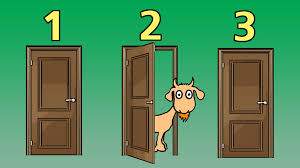
\includegraphics[scale=0.5]{MontyHall.jpg}
\caption{Monty Hall Problem}
\end{figure}
\end{frame}

\begin{frame}
\begin{figure}
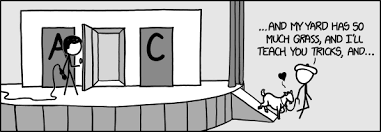
\includegraphics[scale=0.5]{xkcdMontyHall.png}
\caption{Or there's another solution...}
\end{figure}
\end{frame}


\begin{frame}{Recap of Last Class}
\begin{itemize}
\item Talked about cardinality
\item Did some examples of the pigeonhole principle
\item Showed that the integers, even integers, odd integers, and rational numbers all have the same cardinality
\item But we showed that the real numbers have a LARGER cardinality than the integers
\end{itemize}
\end{frame}

\begin{frame}{More Cardinality}
\begin{itemize}
\item Now: we'll show that the power set of $A$ always has a larger cardinality than $A$.
\item $|A|<|P(A)|$
\item Examples:
\begin{enumerate}
\item $A = \{1,2\}, P(A) = \{\emptyset, \{1\}, \{2\}, \{1,2\}\}$, $|A|=2, P(A)=4$
\item $P(\emptyset) = \{\emptyset\}$, $|\emptyset| = 0, |\{\emptyset\}| = 1$
\end{enumerate}
\end{itemize}
\end{frame}

\begin{frame}{Axiom of Choice}
\begin{itemize}
\item Given any set of mutually disjoint nonempty sets, there exists at least one set that contains exactly one element in common with each of the nonempty sets.
\item \textit{The Axiom of Choice is necessary to select a set from an infinite number of pairs of socks, but not an infinite number of pairs of shoes}
\item Implication: Banach-Tarski
\end{itemize}
\end{frame}

\begin{frame}{Zorn's Lemma}
\begin{itemize}
\item If $S$ is any nonempty partially ordered set in which every chain has an upper bound, then $S$ has a maximal element.
\end{itemize}
\end{frame}

\begin{frame}{The Well-Ordering Principle}
\begin{itemize}
\item \textit{The Axiom of Choice is obviously true, the well-ordering principle is obviously false, and who can tell about Zorn's Lemma?}
\item Well-ordering principle: Every set can be well-ordered
\item What is a well-ordering? It means that we order the elements in such a way such that every subset has a least element
\end{itemize}
\end{frame}

\begin{frame}{Induction}
\begin{itemize}
\item If a fact is true about 0, and if whenever it's true about $n$, then it's also true about $n+1$, then it's true about every integer.
\item $\sum_{i=1}^n n = \frac{n(n+1)}{2}$
\item If $n$ lines are drawn in the plane and no two lines are parallel, how many regions do they separate the plane into?
\end{itemize}
\end{frame}

\begin{frame}{Next Time}
\begin{itemize}
\item Transfinite Induction
\item Goodstein's Theorem
\end{itemize}
\end{frame}

\end{document}